Amplitude modulation (AM) is well-studied~\cite{rappaport} and is used in numerous communications systems. AM communications rely on carefully designed transmitters and thoroughly regulated allocation of the frequency spectrum to minimize interference. Unintentional AM signals in computer systems are generated by many possible ``transmitters.'' A memory clock signal, for example, may act as a carrier. A clock signal creates periodic currents at the clock frequency $f_c$, and these currents flow through power and signal wires, generating a strong EM field. When the memory is active, more current is drawn by the clock, and less current is drawn when the memory is less active. If we alternate between high memory activity and low memory activity with a frequency $f_{alt}$, the amplitude of the carrier at $f_c$ is modulated creating signals at $f_c \pm f_{alt}$.

The transmission and reception of such unintentional modulation ``signals'' differ from communication signals in several ways. Since unintentional signals occur at the frequency of the unintentional carrier, they are mixed in with all the other noise generated by the computer system (other clocks and switching noise) and other communications signals. Unintentional signals are subject to EMC restrictions which impose a maximum noise power (signal power from our point of view). Therefore, unintentional signals are typically weaker and may be diffused across the spectrum by spread spectrum clocking or by using clock sources with inherent variation (e.g. RC oscillators). Also, since the carriers are typically generated by non-sinusoidal sources, the carrier signals may have harmonics.

These effects complicate the detection of unintentionally modulated signals. The presence of noise generated by the system makes it difficult to determine which signals are AM carriers and sidebands. Some of the unintentional AM carriers are generated by spread spectrum clocked signals, making them harder to recognize. Existing methods to find AM modulation based on its spectral properties (i.e. without knowing the baseband signals) are not designed to deal with these issues.

Finally, communication signals have direct and obvious control of the baseband (modulation) signal while unintentionally modulated signals from computer systems do not. In some cases, multiple baseband signals may even modulate the same unintentional carrier present in a computing system. We may, for example, be interested in separating out and determining the source of each such baseband signal (i.e. a particular system activity). For example, a baseband signal may be caused by processor activity and another baseband signal may be caused by memory activity. Existing AM detection methods are not able to identify which carriers are modulated by specific system activities.

The spectral properties of amplitude modulated non-ideal carriers are summarized in Section~\ref{am_spectra}. Several other non-ideal properties of computer systems are seen in measured spectra. Randomly timed switching activity causes broadband noise, and this noise appears as gently rolling ``hills'' and ``valleys'' in the spectrum. Additionally, a realistic spectrum contains periodic signals from both inside and outside the system that are either not modulated at all or that \emph{are} AM-modulated (e.g. AM radio broadcasting) but not by program activity. Such a spectrum is shown in Figure~\ref{am_details_e}. Even if we know the carrier and the program activity's frequency content it is hard to decide whether this spectrum contains an activity-modulated signal by visual inspection. Our FASE methodology uses several specially generated program activities in conjunction with a heuristic carrier likelihood
%\footnote{Likelihood here does not refer to probability estimates.}
function to automate the decision process and overcome these problems.

\begin{figure}[thb]
  \centering
    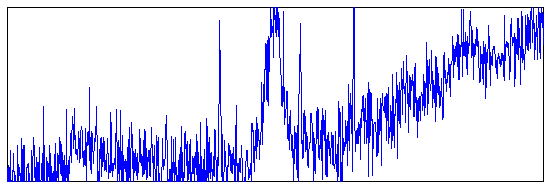
\includegraphics[scale=.95]{../fase/Data/am_details_e.pdf}
  \caption{The same non-ideal carrier and arbitrary side-band signal as Figure~\ref{am_details_d} with noise and other sources present.}
  \label{am_details_e}
\end{figure}

Many periodic carrier signals in computer systems are generated by digital circuits and clocks, and therefore have sharp transitions that are best approximated by rectangular pulses instead of the sinusoidal waves used as carriers in communications systems. The spectrum of a pulse train with an arbitrary duty cycle is equivalent via Fourier analysis to a set of sinusoids with various amplitudes at $f_c$ and its multiples (harmonics). 
In other words, for each carrier signal generated by a digital circuit or clock, additional carrier signals will also be present at $2f_c$, $3f_c$, $4f_c$, $5f_c$, etc. As the duty cycle of a signal approaches 50\%, the amplitudes of the odd-numbered harmonics ($f_c$, $3f_c$, $5f_c$, etc.) reach their maximum, while amplitudes of the even harmonics ($2f_c$, $4f_c$, etc) trend toward zero. For a small duty cycle (i.e. $<$ 10\%), the magnitudes of the first few harmonics (both even and odd) decay approximately linearly. Finally, note that these observations imply that the amplitudes of all the harmonics are a function of the duty cycle. If program activity modulates the duty cycle of a periodic signal while keeping its period constant (i.e. causes pulse width modulation), all of the signal's harmonics are amplitude-modulated and consequently will be identified by our FASE methodology.

